
\documentclass[11pt,a4paper]{article}

\usepackage[utf8]{inputenc}
\usepackage[T1]{fontenc}
\usepackage{lmodern}
\usepackage{amsmath, amssymb, amsthm}
\usepackage{geometry}
\geometry{margin=1in}
\usepackage{tcolorbox}
\usepackage{minted}
\usepackage{booktabs}
\usepackage{tabularx}
\usepackage{tikz}
\usetikzlibrary{shapes.geometric, arrows.meta, positioning}

% Custom environment for important definitions and theorems
\newenvironment{important}{
    \vspace{1em}
    \begin{tcolorbox}[colback=blue!5!white, colframe=blue!75!black, boxrule=1pt, arc=4pt, left=10pt, right=10pt, top=10pt, bottom=10pt]
}{
    \end{tcolorbox}
    \vspace{1em}
}

% Custom command for exam-relevant / critical remarks
\newcommand{\sta}{\textbf{[\textasteriskcentered\ CRITICAL NOTE:] }}

\setlength{\parindent}{0pt}
\setlength{\parskip}{0.8em}

\begin{document}
% Lecture Notes: Biological Background and DNA Sequencing Technology

\section{Introduction to Bioinformatics}

Bioinformatics is an interdisciplinary field that develops methods and software tools to understand complex and large biological datasets. It is important to distinguish the core focus of bioinformatics from related computational fields. 

\begin{important}
    \textbf{Bioinformatics}: The science of information and information flow in biological systems, utilizing mathematical, statistical, and computing methods to solve biological problems using DNA, RNA, and amino acid sequences.
\end{important}

While bioinformatics requires strong programming and computer science foundations, it is essentially an \textit{information science} applied to biological data. This entails the analysis, classification, manipulation, storage, retrieval, and transmission of biological information stored in living cells. Furthermore, bioinformatics is not strictly the study of biologically-inspired computational models (like artificial neural networks or genetic algorithms), though it may employ these models as tools to analyze biological data.

Most bioinformatics analyses are performed \textit{in silico} (computationally), utilizing data gathered \textit{in vivo} (from living organisms) or \textit{in vitro} (from lab environments, such as petri dishes).

\section{Molecular Biology Foundations}

To properly analyze genomic data, one must understand how the underlying biological machinery stores and processes information. 

\subsection{Cells and Macromolecules}
Cells are the fundamental working units of every living system. We broadly classify cells into:
\begin{itemize}
    \item \textbf{Prokaryotic cells} (e.g., bacteria): The genetic material (DNA) is "free-floating" in the cellular fluid (cytoplasm) and is typically a single circular genome.
    \item \textbf{Eukaryotic cells} (e.g., animals, plants): The DNA is packaged into multiple chromosomes and enclosed within a defined \textbf{nucleus}.
\end{itemize}

% [IMAGE: Microscopic view and simple diagram comparing Prokaryotic and Eukaryotic cells, highlighting the presence of a nucleus in Eukaryotes.]

Within these cells exist small molecules (water, sugars, fatty acids) and \textbf{macromolecules}, which are large, complex structures built from smaller units. The primary macromolecules of interest in bioinformatics are:
\begin{enumerate}
    \item \textbf{Proteins}: The functional building blocks of the cell. They catalyze chemical reactions (enzymes), form cellular structures, and transmit signals. Proteins are composed of chains of amino acids.
    \item \textbf{DNA (Deoxyribonucleic acid)}: The primary storage and replication medium for biological information. It contains both genes (protein-coding regions) and regulatory elements. 
    \item \textbf{RNA (Ribonucleic acid)}: A single-stranded molecule that plays a key role in transforming the genetic information stored in DNA into functional proteins.
\end{enumerate}

\section{The Chemical Structure of DNA and RNA}

DNA and RNA are polymers formed by linking simple building blocks called \textbf{nucleotides}. 

\subsection{Nucleotides and the DNA Backbone}
Each nucleotide consists of three chemical components:
\begin{itemize}
    \item A \textbf{phosphate group}
    \item A \textbf{pentose sugar} (deoxyribose in DNA, ribose in RNA)
    \item A \textbf{nitrogen-containing base}
\end{itemize}

The phosphate group and the sugar form the structural "backbone" of the molecule, connected via covalent bonds. The identity of the nucleotide is determined entirely by the nitrogenous base attached to it. 

\begin{important}
    \textbf{The Genetic Alphabet}: The information in DNA is encoded by four bases:
    Adenine (A), Cytosine (C), Guanine (G), and Thymine (T). \\
    In RNA, Thymine (T) is replaced by Uracil (U).
\end{important}

\subsection{Directionality and the Double Helix}
DNA molecules have a strict directionality. The carbon atoms of the pentose sugar are numbered \(1'\) through \(5'\). The phosphate group is attached to the \(5'\) carbon, and the next nucleotide in the chain is added at the \(3'\) carbon (which possesses a free hydroxyl (-OH) group). 

\sta \textbf{Direction of Synthesis and Reading}: Biological systems synthesize and read DNA in the \(5' \to 3'\) direction. Consequently, all sequence data in bioinformatics is conventionally written and interpreted in the \(5' \to 3'\) direction.

DNA exists as a \textbf{double helix}: two complementary strands wrapped around each other. These strands exhibit two critical structural properties:
\begin{enumerate}
    \item \textbf{Anti-parallel orientation}: The two strands run in opposite directions. If one strand runs \(5' \to 3'\), the opposite strand runs \(3' \to 5'\).
    \item \textbf{Base Pairing}: The two strands are held together by hydrogen bonds between the bases. Due to chemical constraints, Adenine (A) always pairs with Thymine (T), and Cytosine (C) always pairs with Guanine (G).
\end{enumerate}

\subsection{The Reverse Complement}
The relationship between the two strands of a DNA molecule is purely deterministic: knowing one strand dictates the exact sequence of the other. Because biological databases typically only store one reference strand to save space, bioinformatics algorithms must frequently compute the corresponding second strand.

\begin{important}
    \textbf{Reverse Complement}: To find the sequence of the opposite DNA strand in the correct \(5' \to 3'\) orientation, one must:
    \begin{enumerate}
        \item \textbf{Complement} the sequence: Swap A with T, T with A, C with G, and G with C.
        \item \textbf{Reverse} the sequence: Flip the order of the characters to reflect the \(5' \to 3'\) reading direction.
    \end{enumerate}
\end{important}

\textbf{Example:} Computing the reverse complement of a short DNA fragment.
\begin{minted}{text}
Positive strand (5' to 3'):   A G T C A G T T A C T A G
Complement string:            T C A G T C A A T G A T C
Reverse Complement (5' to 3'):C T A G T A A C T G A C T 
\end{minted}

The above plain-text block demonstrates the exact sequence of steps. First, we identify the complement of each individual base. Because the matching complementary strand is physically anti-parallel (running \(3' \to 5'\) relative to our left-to-right reading), we must reverse the final string so that it can also be read conventionally from \(5'\) to \(3'\). 

\sta This property allows DNA replication: a cell can separate the double helix and use each individual strand as a template to synthesize its missing reverse complement, resulting in two identical double-stranded DNA molecules.

\section{The Central Dogma of Molecular Biology}

The "Central Dogma" describes the flow of genetic information within a living cell, from the storage medium (DNA) to the functional product (proteins).

\begin{center}
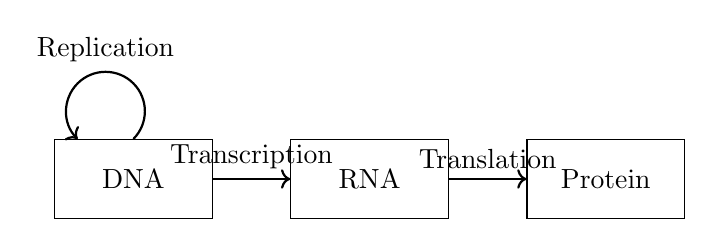
\begin{tikzpicture}[node distance=3cm, auto]
    \node (dna) [draw, rectangle, minimum width=2cm, minimum height=1cm] {DNA};
    \node (rna) [draw, rectangle, right of=dna, minimum width=2cm, minimum height=1cm] {RNA};
    \node (protein) [draw, rectangle, right of=rna, minimum width=2cm, minimum height=1cm] {Protein};

    \draw [->, thick] (dna) -- node {Transcription} (rna);
    \draw [->, thick] (rna) -- node {Translation} (protein);
    \draw [->, thick] (dna.north) arc [start angle=-45, end angle=225, radius=0.5cm] node[midway, above] {Replication};
\end{tikzpicture}
\end{center}

\subsection{Transcription and RNA Splicing}
\textbf{Transcription} is the process by which an RNA polymerase enzyme creates a single-stranded RNA copy from a DNA template. As the lecturer noted intuitively, this is similar to a medieval monk manually copying a master text into a new book. The resulting molecule is a pre-messenger RNA (pre-mRNA).

In eukaryotes, transcription occurs inside the nucleus, but translation occurs outside in the cytoplasm. This separation allows the cell to post-process the pre-mRNA before it is translated, a process known as \textbf{RNA splicing}.
\begin{itemize}
    \item \textbf{Introns} are intervening sequences that are "spliced out" (removed and discarded).
    \item \textbf{Exons} are the remaining sequences that are ligated together to form the mature mRNA.
\end{itemize}

\textbf{Alternative Splicing}: A single pre-mRNA can be spliced in multiple different ways (e.g., by entirely skipping an exon). This flexibility allows a single gene to code for multiple different protein variants, explaining why organisms like humans can be highly complex despite having a relatively low total gene count compared to some plants like rice.

% [IMAGE: Diagram showing a pre-mRNA strand with alternating Exons (colored) and Introns (grey), followed by multiple mature mRNA variants formed by selecting different combinations of Exons (Alternative Splicing).]

\subsection{Translation}
\textbf{Translation} is the synthesis of a protein from the mature mRNA transcript, carried out by ribosomes in the cytoplasm. 

Because there are only 4 RNA bases (A, C, G, U) but 20 functional amino acids, the genetic code is read in non-overlapping triplets called \textbf{codons}. 
\begin{itemize}
    \item 3 bases provide \(4^3 = 64\) possible combinations, allowing for redundancy.
    \item \textbf{Start Codon}: The sequence \texttt{AUG} signals the ribosome to start translating and establishes the reading frame.
    \item \textbf{Stop Codons}: Sequences like \texttt{UAA}, \texttt{UAG}, or \texttt{UGA} signal the termination of the protein chain.
\end{itemize}
Transfer RNA (tRNA) molecules carry specific amino acids to the ribosome, binding to the mRNA codons via their own reverse-complementary "anti-codons". The amino acids are joined sequentially via peptide bonds, building the polypeptide chain from the N-terminus (amino group) to the C-terminus (carboxyl group).

\section{Systems Biology and "Omics"}
The cellular system is incredibly complex, driven by intertwined signaling pathways and metabolic processes. To understand the entire state of a biological system rather than isolated parts, high-throughput technologies are used to study the complete set of specific biological molecules:
\begin{itemize}
    \item \textbf{Genomics}: Study of the genome (the complete set of DNA).
    \item \textbf{Transcriptomics}: Study of the transcriptome (the complete set of RNA transcripts, indicating which genes are currently "expressed" or turned on).
    \item \textbf{Proteomics}: Study of the proteome (the complete set of proteins).
\end{itemize}

\section{DNA Sequencing Technologies}
To perform genomic and transcriptomic analyses, we must be able to read the exact sequence of nucleotide bases in a biological sample.

\subsection{Sanger Sequencing (First Generation)}
Developed by Fred Sanger, this method is known as \textbf{sequencing by synthesis}.

\begin{important}
    \textbf{Sequencing by Synthesis (Sanger Method)}: A technique that determines a DNA sequence by reconstructing its complementary strand and observing which specific nucleotide is added at every step.
\end{important}

\textbf{Mechanism:}
\begin{enumerate}
    \item The double-stranded DNA is separated, and one strand is used as a template.
    \item A mixture of standard nucleotides (dNTPs) and modified \textbf{chain-terminating dideoxynucleotides (ddNTPs)} is introduced. These ddNTPs lack the \(3'\)-OH group required to attach the next nucleotide.
    \item When the DNA polymerase accidentally incorporates a ddNTP instead of a standard nucleotide, synthesis halts entirely.
    \item This creates a massive pool of DNA fragments of every possible length, each ending at the specific nucleotide where termination occurred.
    \item \textbf{Electrophoresis}: The fragments are pulled through a gel using an electric current. Smaller fragments travel faster than larger ones. By arranging them by length, the sequence can be read sequentially.
\end{enumerate}

Originally, the four terminating nucleotides were labeled with radioactive isotopes and run in four separate parallel lanes. Modern Sanger sequencing utilizes \textbf{fluorescent dyes} (a different color for A, C, G, and T), allowing the fragments to be run in a single lane and read automatically by a laser to produce a chromatogram. While highly accurate, Sanger sequencing has a very low throughput.

% [IMAGE: A sequence chromatogram graph showing a series of colored peaks (red, green, blue, black) plotted over time, each representing a base (A, T, C, G) identified as fragments pass a laser detector.]

\subsection{Next-Generation Sequencing (Illumina)}
To vastly increase throughput and lower costs, Next-Generation Sequencing (NGS) massively parallelizes the synthesis process. The dominant technology (Illumina) handles millions of short fragments simultaneously.

\textbf{Step 1: Library Preparation}
\begin{enumerate}
    \item \textbf{Fragmentation}: Genomic DNA is randomly sheared into short, uniform fragments (typically <800 bp).
    \item \textbf{End Repair \& A-Tailing}: The broken ends of the double helix are chemically smoothed, and a single 'A' nucleotide is appended to the \(3'\) ends.
    \item \textbf{Adapter Ligation}: Synthetic DNA segments called \textbf{adapters} (which end with a 'T' overhang) are ligated to both ends of the fragments. These adapters serve as known biological "handles" for unknown sequences.
\end{enumerate}

\textbf{Step 2: Flow Cell Preparation and Bridge Amplification}
The library is washed over a "flow cell," a glass slide coated with short sequences that are reverse-complementary to the adapters.
\begin{enumerate}
    \item The fragments attach to the flow cell via the adapters.
    \item To strengthen the chemical signal, a process called \textbf{bridge amplification} is performed. The attached fragments arch over and attach their free end to a neighboring site, forming a bridge. 
    \item The DNA is copied, creating a local cluster of identical DNA fragments (roughly 1,000 identical copies per original fragment).
\end{enumerate}

\textbf{Step 3: Sequencing by Synthesis (Reversible Terminators)}
\begin{enumerate}
    \item The sequencer floods the flow cell with all four fluorescently labeled nucleotides. 
    \item Unlike Sanger's permanent terminators, NGS uses \textbf{reversible terminators}. Only one nucleotide can be added to the growing chain before synthesis stops.
    \item A laser excites the flow cell. A camera records the color emitted by each distinct cluster on the slide, identifying the exact base just added.
    \item The terminator block is chemically removed, and the cycle repeats.
\end{enumerate}

\textbf{Limitations of NGS:}
The sequencing read length is restricted (typically 300-500 base pairs). As cycles progress, stochastic failures occur (e.g., a fragment in a cluster fails to attach a nucleotide in one round). Over hundreds of cycles, this desynchronization creates background noise that ultimately drowns out the primary light signal, terminating the read.

\subsection{Third-Generation Sequencing (Nanopore)}
To address the short-read limitation, technologies like Oxford Nanopore sequence single, long DNA molecules directly.

\textbf{Mechanism}: A single DNA strand is pulled through a microscopic protein pore (nanopore) embedded in a membrane. A continuous voltage is applied. As different bases (A, C, G, T) pass through the pore, they obstruct the flow of ions to different extents, creating characteristic changes in the electrical current.

\textbf{Trade-offs}:
\begin{itemize}
    \item \textbf{Pros}: Generates massively long reads (e.g., 10,000 to over 100,000 base pairs). Crucial for assembling highly repetitive genomes where short reads fail to provide unique contextual overlaps.
    \item \textbf{Cons}: Historically higher error rates compared to Sanger and Illumina, largely due to electrical signal-to-noise ratios, though continually improving.
\end{itemize}

\subsection{Applications Beyond Genomics}
While these technologies are designed to sequence DNA, they are incredibly versatile:
\begin{itemize}
    \item \textbf{RNA-Seq}: To measure gene expression, RNA is extracted and reverse-transcribed into complementary DNA (cDNA). The cDNA is then sequenced on standard Illumina machines.
    \item \textbf{ChIP-Seq (Chromatin Immunoprecipitation Sequencing)}: Used to find where specific proteins bind to the genome. DNA is cross-linked to bound proteins, chopped into pieces, and isolated using targeted antibodies. The captured DNA is stripped from the proteins and sequenced, mapping the protein's exact binding locations.
\end{itemize}

\end{document}
